% The first part of this file defines the Feynman diagram
% (for now the same as in presentation/feynman_higgsstrahlung.tex).
% Then, the Feynman diagram is combined with some figures into a schematic.

% Define styles for the different kind of edges in a Feynman diagram
\tikzset{
    vector/.style={decorate, draw=black,
    decoration={snake, segment length=4mm, amplitude=1mm}},
    fermion/.style={draw=black, postaction={decorate},
        decoration={markings,mark=at position .55 with {\arrow[draw=black]{>}}}},
    fermionbar/.style={draw=black, postaction={decorate},
        decoration={markings,mark=at position .55 with {\arrow[draw=black]{<}}}},
    gluon/.style={decorate, draw=black,
        decoration={coil,amplitude=4pt, segment length=5pt}},
    higgs/.style={dashed,draw},
    photon/.style={decorate, decoration={snake}, draw=black},
    electron/.style={draw=black, postaction={decorate},
        decoration={markings,mark=at position .55 with {\arrow[draw=black]{>}}}},
    positron/.style={draw=black, postaction={decorate},
        decoration={markings,mark=at position .55 with {\arrow[draw=black]{<}}}}
}

\newcommand{\DrawFeynman}{
    \node (i1 e+) at (-140:2) {};
    \node (v4 ISR) at (-140:1.5) {};
    \begin{scope}[shift={(v4 ISR)}]
        \node (f4 gamma) at (10:1.5) {};
    \end{scope}
    \node (i2 e-) at (140:2) {};

    \node (v1 eeZ) at (0,0) {};
    \node (v2 ZZH) at (0:2) {};
    \begin{scope}[shift={(v2 ZZH)}]
        \node (v3 Zll) at (-40:1.5) {};
        \node (f1 H) at (40:1.6) {};
    \end{scope}
    \begin{scope}[shift={(v3 Zll)}]
        \node (f3 l-) at (-60:2) {};
        \node (f2 l+) at (-20:2) {};
        \node (v5 FSR) at (-20:0.5) {};
    \end{scope}
    \begin{scope}[shift={(v5 FSR)}]
        \node (f5 gamma) at (0:1.5) {};
    \end{scope}
    \begin{scope}[shift={(f3 l-)}]
        \node (f6 nu tau) at (-10:1.5) {};
        \node (f7 W) at (10:1.5) {};
    \end{scope}


    \draw[fermionbar] (i1 e+)--(v1 eeZ.center);
        \node at (i1 e+) {$e^+$};
    \draw[fermion] (i2 e-)--(v1 eeZ.center);
        \node at (i2 e-) {$e^-$};

    \draw[vector] (v1 eeZ.center)--(v2 ZZH.center);
        \node at ($ 0.5*(v1 eeZ) + 0.5*(v2 ZZH)  + (0,0.3) $) {$Z$};
    \draw[vector] (v2 ZZH.center)--(v3 Zll.center);
        \node at ($ 0.5*(v2 ZZH) + 0.5*(v3 Zll)  + (0.2,0.2) $) {$Z$}; % = midpoint of propagator + fine tuning
    \draw[higgs] (v2 ZZH.center)--(f1 H);
        \node at (f1 H) {$H$};

    % \draw[vector] (v4 ISR.center)--(f4 gamma);
    % \node at (f4 gamma) {$\gamma$};

    \draw[fermion] (v3 Zll.center)--(f3 l-);
    \draw[fermionbar] (v3 Zll.center)--(f2 l+);

    \node at (f3 l-) {$l^-$};
    \node at (f2 l+) {$l^+$};
    \draw[vector] (v5 FSR.center)--(f5 gamma);
    \node at (f5 gamma) {$\gamma$};
}

\tikzset{
    every path/.append style={line width=0.05cm,},
    box/.style={draw=C3,rounded corners,line width=0.1cm,},
}
\newcommand{\RectPad}{0.4}
\newcommand{\StepTitle}[1]{
    {\normalsize\color{C3}#1}
}
\newcommand{\StepBox}[2]{
    \begin{tabular}{l}
        \StepTitle{#1}\\
        {\footnotesize\hspace{1em}
            \begin{tabular}{l}
            #2
            \end{tabular}
        }
    \end{tabular}
}
\newcommand{\EventSelectionText}{
    \StepBox{1. Event selection:}
        {$M_{\mathrm{recoil}}^2 = s + M_Z^2 - 2\sqrt{s} \cdot E_Z$}
}
\newcommand{\SampleSelectionText}{
    \StepTitle{2. Sample creation}
}
\newcommand{\BRFitText}{
    \StepBox{3. BR fit:}{
        Probability matrix M from simulation\\
        per bkg and decay mode. \\
        Minimize $ BR = M \cdot Data$
    }
}


\begin{block}{Schematic overview}
    \vspace{1em}
    \resizebox{\textwidth}{!}{
    \scriptsize
    \begin{tikzpicture}[remember picture]
        \DrawFeynman

        % The event selection box.
        \node[anchor=west] (ev_sel) at (f2 l+.east) {\EventSelectionText};
        \path let \p1=(ev_sel.south east),\p2=(f3 l-.south) in coordinate (box 1 lower left) at (\x1, {min(\y1,\y2)});
        \draw[box] ($(v3 Zll.west) + (\RectPad,\RectPad)$) rectangle ($(box 1 lower left) + (\RectPad,-\RectPad)$) {};

        % The sample creation box
        \node[anchor=south] (sample img) at ($(f1 H.north) + (\RectPad, 0)$) {
            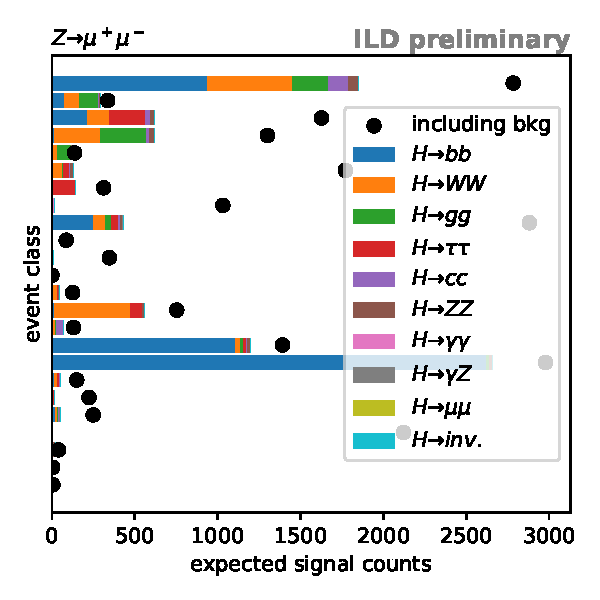
\includegraphics[height=10cm]{intro_category_counts_w_bkg}
        };
        \node[anchor=center] (sample txt) at (sample img.north) {\SampleSelectionText};
        \path let \p1=(sample txt.north east),\p2=(sample img.north east) in coordinate (box 2 upper right) at ({max(\x1,\x2)},\y1);
        \path let \p1=(f1 H.south),\p2=(sample img.west) in coordinate (box 2 lower left) at (\x2,\y1);
        \draw[box] ($(box 2 upper right) + (\RectPad,\RectPad)$) rectangle ($(box 2 lower left) + (\RectPad,-\RectPad)$) {};

        % The BR fit step
        \node[anchor=north west] (fit txt) at ($(box 2 upper right) + 4*(\RectPad,0)$) {\BRFitText};
        \node[anchor=north west] (fit matrix) at (fit txt.south west) {
            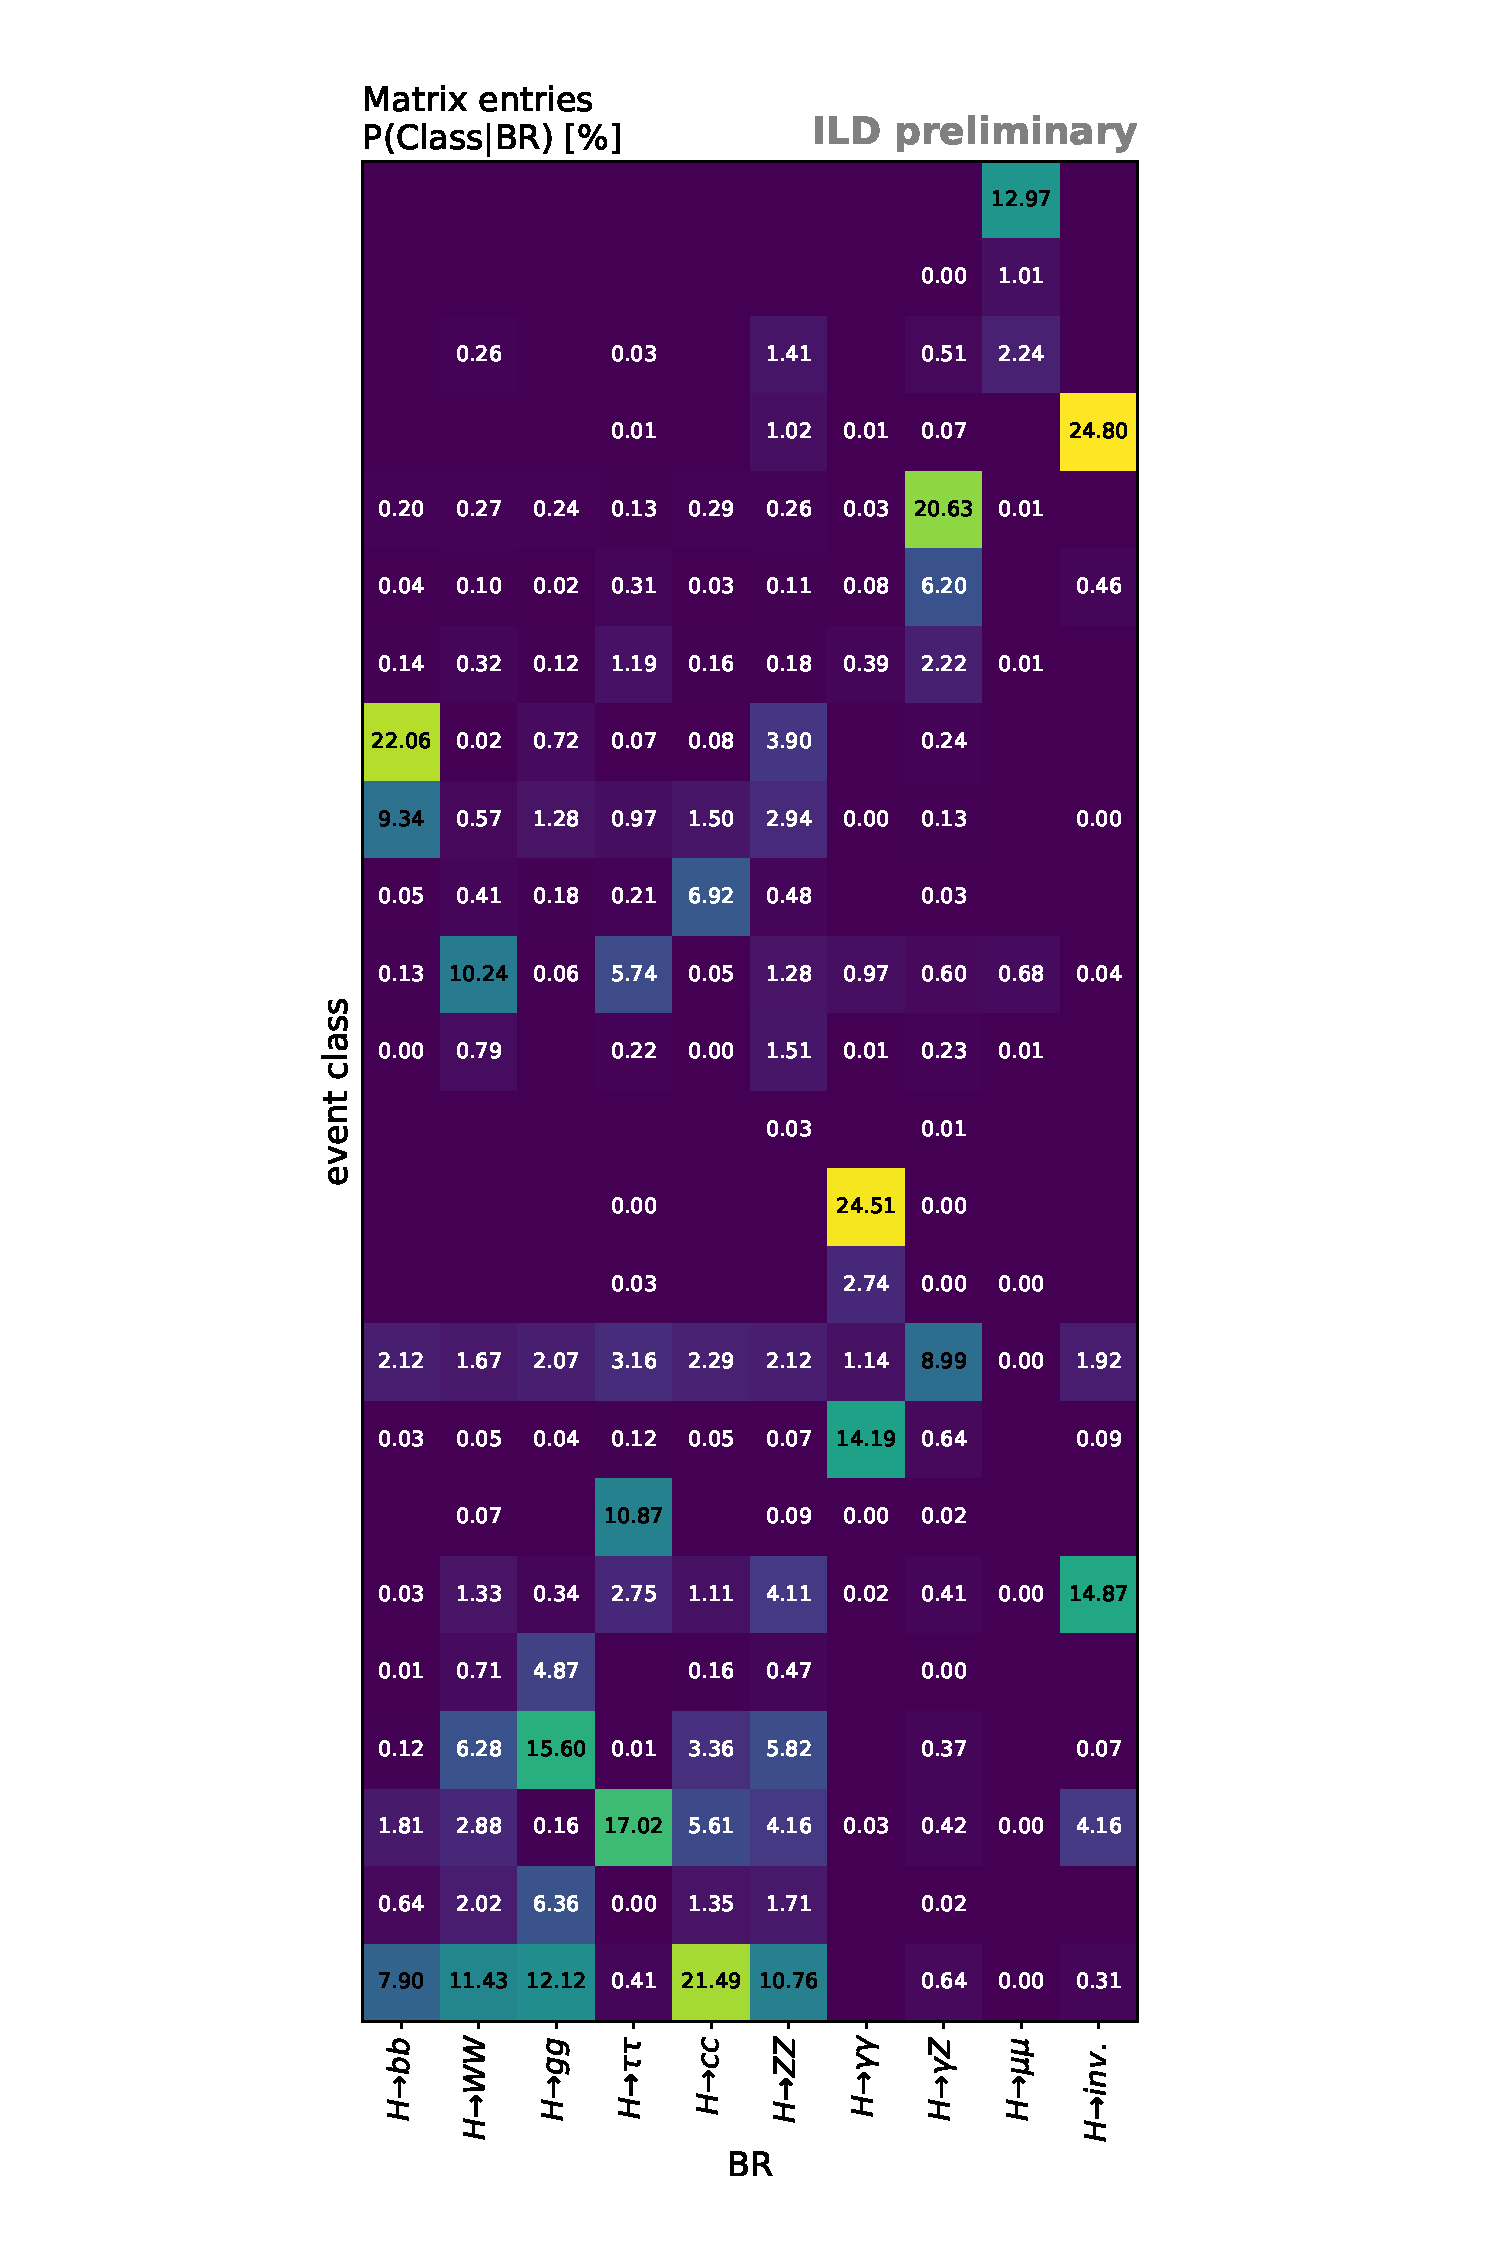
\includegraphics[height=8cm]{probability_matrix}
        };
        \path let \p1=(fit txt.north east),\p2=(fit matrix.south east) in coordinate (box 3 lower right) at ({max(\x1,\x2)},\y2);
        \draw[box] ($(fit txt.north west) + (-\RectPad,\RectPad)$) rectangle ($(box 3 lower right) + (\RectPad,-\RectPad)$) {};
        \path let \p1=(sample txt.north east),\p2=(sample img.east) in coordinate (arrow start) at ({max(\x1,\x2)},\y2);
        \draw[-{Triangle[width=18pt,length=8pt]}, line width=8pt](arrow start) -- ($(arrow start) + 4*(\RectPad, 0)$);
      \end{tikzpicture}
    }
    \vspace{0em}
\end{block}
